% Document title
% ==============
% Draft for conference/workshop paper to be submitted to http://tappcs.blogspot.mx/
% 2--4 pages in Spanish or English.

\documentclass[10pt,conference,a4paper]{IEEEtran}
\usepackage[utf8x]{inputenc}
\usepackage[hidelinks]{hyperref}
\usepackage{graphicx}
\usepackage{pgfplots}
\usepackage[T1]{fontenc}
\bibliographystyle{IEEEtran}

% This enables the kanji in the table, but all typefaces turn uglier.
% Also must be generated with xelatex
%\usepackage{xeCJK}
%\setCJKmainfont{cyberbit.ttf}


\title{Some Nice Title Goes Here, Eventually\ldots}

\author{
	\IEEEauthorblockN{Lars Fredrik Karlstr\"om}
	\IEEEauthorblockA{Faculty of Science, Dept. of Computer Science\\ Universidad Aut\'onoma de Baja California\\ \href{mailto:fredrik.karlstrm@uabc.edu.mx}{\texttt{fredrik.karlstrm@uabc.edu.mx}}}
	\and
	\IEEEauthorblockN{Dr. Everardo Guti\'errez L\'opez}
	\IEEEauthorblockA{Faculty of Science, Dept. of Computer Science\\ Universidad Aut\'onoma de Baja California\\ \href{mailto:everardo.gutierrez@uabc.edu.mx}{\texttt{everardo.gutierrez@uabc.edu.mx}}}
}

\pgfplotsset{
	compat = newest,
	xlabel near ticks,
	ylabel near ticks
}

%\markboth{TACS 2014 and more info here}{} % Only on journal papers, apparently...

\begin{document}
	\maketitle

	\begin{abstract}
		Quick content summary.
		Motivation. (From 'Robust': High accuracy has been attained, but speedup/size improvements still important for mobile and desktop.)
	\end{abstract}
	\medskip
	\begin{IEEEkeywords}
		Intelligent character recognition, artificial neural network, handwriting recognition, Japanese writing, \ldots
	\end{IEEEkeywords}


	\section{Problem description}

	Any form of digital handwriting recognition is a complex undertaking,
	where the performance of the system is impacted by a multitude of factors -- spanning
	everything from the quality and quantity of training data, to resilience toward input
	translation, rotation, and noise. As the number of candidate categories increases
	the size of the search space, however, the task quickly grows monumental.

	The Japanese writing system consists of the two \emph{kana} syllabaries \emph{hiragana} and \emph{katakana},
	as well as the sinographs commonly known as \emph{kanji} -- literally ``Han characters'' -- that stem from China.
	The Japanese Ministry of Education's official ``regular use'' (j\=oy\=o) kanji list defines a set of 2,136
	baseline characters taught in elementary-- and secondary--school education. \cite{hadamitzky2012japanese} This set is far from exhaustive, though:
	the Japanese Industrial Standard X 0208 encoding, for instance, contains 6,355 different kanji.

	Given that the category search space for Japanese characters is an order of magnitude larger than its western counterparts,
	it becomes apparent that a monolithic system design would be both unwieldly and computationally expensive, requiring
	deep neural networks \cite{ciresan2012multi} to attain high recognition rates.

	In this work, we describe a flexble, modular design scheme that splits the identification task into coarse and fine steps,
	thereby reducing the complexity of each component. The design scheme also permits replacing classification strategies,
	and facilitates the parallelization of network training.

	 
	\section{Previous work}

	Testing a cite \cite{zhu2014robust}.

	\ldots

	In \cite{nakai2001substroke}, the authors adapt a continuous speech recognition algorithm utilizing
	hidden Markov models for the purpose of online kanji recognition. By identifying and classifying
	substrokes, which in turn are employed as search keys in a character dictionary, this approach vastly
	reduced the memory requirements for both their models and their dictionary.


	``Online Handwritten Kanji Recognition Based on Inter-stroke Grammar'' uses the A-H0-9 classification scheme,
	and discusses the hierarchical structure of kanji.

	``A linear--time elastic matching algorithm for on--line recognition of handwritten Japanese characters'' (Nakagawa)
	presents the LTM--algorithm, an alternative and attractive way of extracting feature points.

	Should we mention alternative solutions, such as SVMs? Tomoe does quite a good job, for instance. Not sure if there
	are academic evaluations/references, though.



	\section{Proposed solution}

	Some text here, followed by a diagram. Divide and conquer!

	\begin{figure}
		\centering
		
\includegraphics[width=2.75in]{./fig/model-overview.eps}
		\caption{Model overview. The input is first analyzed by the coarse classifier, resulting in the $<GHA\ldots>$ feature representation.
		Thereafter, the routing network selects which cluster to search in, and the image data is passed to the corresponding CANN for fine--grain classification.}
		\label{fig_model_overview}
	\end{figure}

	\subsection{Feature extraction}

	\subsection{Category clustering}

	As is proven in \cite{drineas2004clustering}, this is an NP-hard problem even in the case of $k = 2$. 

	Centroid-based clustering
	"Seeks to minimize the average squared distance between points in the same cluster"
	goal is to choose k centers so as to minimize $\varphi$, the total squared distance between each point and its closest center.

	\subsection{Feedforward routing network}

	\subsection{Convolutional character classification network}


	\section{Experiments}

	This will be a short section\ldots
	Describe the simple online feature extractor and following clustering scheme.

	\ldots

	Whereas in \cite{nakai2001substroke} strokes were segmented into substrokes and classified in
	25 dimensions, our initial feature extraction strategy provides a coarse full--stroke classification
	in 8 dimensions. By discarding ``pen--up motions,'' we render the system more resilient to erroneous
	stroke order, at the cost of increasing variability within each cluster.

	\subsection{Clustering}

	\ldots decided to consider the value given by the ``rule of thumb'' $k \approx \sqrt{n / 2}$ proposed in \cite{mardia2005multivariate}
	as an upper limit to the number of clusters.

	$$ k_{max} = \sqrt{6,396 / 2} \approx 57 $$

	The clusters were generated using the k--means++ algorithm,
	a variation of Lloyd's algorithm that seeks to improve the selection of the initial centroids. \cite{arthur2007k}



Total strokes: 78785

\begin{table}
	\renewcommand{\arraystretch}{1.3}
	\caption{Statistical overview of \ldots}
	\label{tbl_stroke_analysis}
	\centering
	\begin{tabular}{ c | c c c c c l }
		\hline
		  & \bfseries \% & \small $\sum$ & $\mu$ & $\sigma$ & Highest count \\ 
		\hline
		\hline
		\bfseries A & $33.20\%$ & $26,160$ & $4.09$ & $2.33$ & $15$ & \\%(蠶) \\
		\bfseries B & $1.47\%$  & $1,159$  & $0.18$ & $0.40$ & $2$  & \\%(摑) \\
		\bfseries C & $0.00\%$  & $0$      & --     & --     & --   & \\%     \\
		\bfseries D & $0.00\%$  & $0$      & --     & --     & --   & \\%     \\
		\bfseries E & $0.31\%$  & $245$    & $0.04$ & $0.19$ & $2$  & \\%(霪) \\
		\bfseries F & $12.72\%$ & $10,018$ & $1.57$ & $1.36$ & $10$ & \\%(鏐) \\
		\bfseries G & $29.98\%$ & $23,616$ & $3.69$ & $1.96$ & $13$ & \\%(鱸) \\
		\bfseries H & $22.32\%$ & $17,587$ & $2.75$ & $1.61$ & $11$ & \\%(靆) \\
		\hline
		\hline
	\end{tabular}
\end{table}



	% Statistical representation was close to perfect after the initial
	% segment of some 3k kanji
	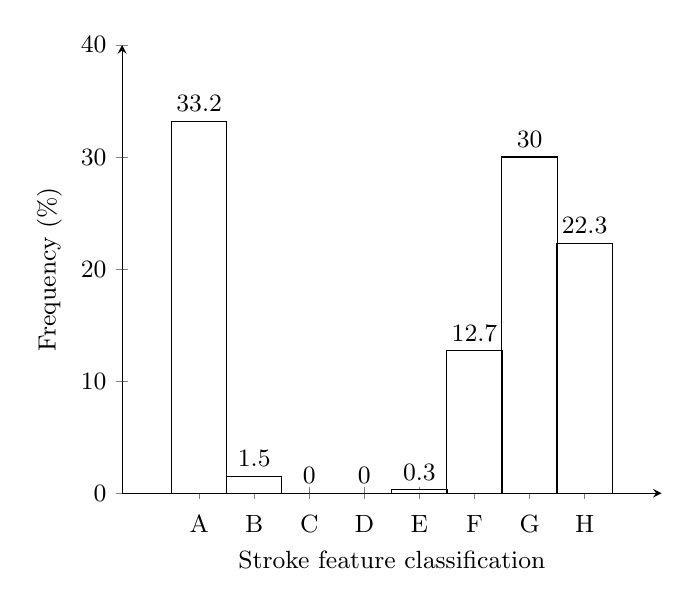
\begin{tikzpicture}[font=\small]
		\begin{axis}[
			ybar,
			bar width=20pt,
			xlabel={Stroke feature classification},
			ylabel={Frequency (\%)},
			ymin=0,
			ymax=40,
			%ytick=\empty,
			xtick=data,
			axis x line=bottom,
			axis y line=left,
			enlarge x limits=0.2,
			symbolic x coords={A, B, C, D, E, F, G, H},
			xticklabel style={anchor=base, yshift=-\baselineskip},
			nodes near coords={\pgfmathprintnumber\pgfplotspointmeta}
		]
			\addplot[fill=white] coordinates {
				(A, 33.2)
				(B, 1.5)
				(C, 0)
				(D, 0)
				(E, 0.3)
				(F, 12.7)
				(G, 30.0)
				(H, 22.3)
			};
		\end{axis}
	\end{tikzpicture}

	\subsection{Preliminary results}

	Not done yet, but here we go.


	\section{Conclusions}

	This work is cool, now give complimentary M.Sc. plx?
	They did it for Donald Knuth\ldots :(


	\section{Future work}

	The experimental results documented in this paper are an initial attempt at applying the proposed methodology;
	numerous variations remain to be explored. With regard to online recognition, the explored feature extraction
	strategy could be enhanced to break strokes into substrokes, diffentiate between long and short strokes, and take
	pen--up movements into account. This alteration would in turn allow clustering on up to 25 dimensions, rather than the current 8.

	By substituting the current coarse classifier with an offline feature extraction strategy, the entire system could
	be evaluated on offline handwriting recognition datasets, such as\ldots. 

	Clustering\ldots

	Finally, at the cluster--specific CANN--level, there is ample opportunity to tweak the network topology as well as
	to apply a variety of best practices \cite{simard2003best} in order to enhance the final, fine--grain recognition results.



	%\section{References}
	\bibliography{./references}

\end{document}
